\chapter{Incapsulare} \label{cap:incapsulare}

\section{Procedure}

Per affrontare l'argomento delle procedure\footnote{In altri contesti, e con modalità funzionali
diverse, lo stesso concetto è realizzato attraverso funzioni, subroutine, metodi.}u riprendiamo il disegno del quadrato, così come lo avevamo fatto usando le variabili (sezione \ref{sec:variabili}):

\vskip 1cm

\begin{scriptsize}
\begin{minipage}{0.40\textwidth}
\begin{itemize}[itemsep=-3pt,parsep=2pt]
\item[] CLEARSCREEN            
\item[] HOME
\item[] 
\item[] LATO = 100
\item[] ANGOLO = 90
\item[] 
\item[] FORWARD LATO
\item[] LEFT ANGOLO
\item[] FORWARD LATO
\item[] LEFT ANGOLO
\item[] FORWARD LATO
\item[] LEFT ANGOLO
\item[] FORWARD LATO
\item[] HIDETURTLE	       
\end{itemize}
\end{minipage}
\end{scriptsize}
\begin{minipage}{0.4\textwidth}
\begin{figure}[H]
   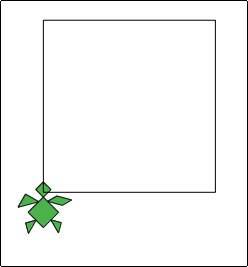
\includegraphics[width=3.0cm,trim=4 4 8 4,clip]{./images/incapsulare/incapsulare-1.png}
   \label{inc-1}
\end{figure}
\end{minipage} \hfill

\vskip 1cm

Abbiamo visto l'utilità delle variabili, ad esempio per cambiare le dimensioni del disegno: se vogliamo fare un quadrato di lato 50 anziché 100 basta cambiare l'istruzione \textbf{LATO = 100} in \textbf{LATO = 50}, invece di cambiare l'argomento di tutte e quattro le istruzioni \textbf{FORWARD}. Tuttavia, se vogliamo disegnare più quadrati, magari di diverse dimensioni e in parti diverse del foglio, dobbiamo riscrivere tutto il blocco di istruzioni, una volta per ogni quadrato. Possiamo ricorrere a alle ripetizioni, in modo da ripetere tutto il blocco di istruzioni, cambiando solo ciò che serve ad ogni ciclo, ma non è detto che si possa ricorrere sempre a questo metodo con profitto. Inoltre, abbiamo già osservato come sia importante scrivere codice chiaro e ordinato. Quasi sempre la concisione è una virtù.  È qui che vengono in aiuto le "subroutine", che in altri linguaggi sono dette "funzioni" e in altri ancora "metodi", ma il concetto di base è lo stesso. L'idea consiste nell'incapsulare una sezione di codice che serva ad un compito ben definito, in modo che questa possano essere impiegata semplicemente invocando una sola istruzione. È un accorgimento straordinariamente potente che consente di semplificare grandemente la scrittura del codice, e di conseguenza, di ridurre la probabilità di commettere errori. 

\vskip 0.5cm

\begin{scriptsize}
\begin{minipage}{0.50\textwidth}
\begin{itemize}[itemsep=-3pt,parsep=2pt, leftmargin=-6.0mm]
\item[] CLEARSCREEN	; operazioni di preparazione                    
\item[] HOME			; che vengono eseguite subito
\item[] SHOWTURTLE
\item[] 
\item[] ; subroutine QUADRATO: viene solo "imparata"...
\item[] 			        ; ma non eseguita
\item[] 
\item[] \color{green}TO \color{red}QUADRATO
\item[] 	\color{blue}LATO = 100	; fisso il lato del quadrato
\item[] 	ANGOLO = 90	; angolo di rotazione ai vertici
\item[] 	FORWARD LATO	; primo lato
\item[] 	RIGHT ANGOLO	; giro di 90\degree a destra, ecc.
\item[] 	FORWARD LATO
\item[] 	RIGHT ANGOLO
\item[] 	FORWARD LATO
\item[] 	RIGHT ANGOLO
\item[] 	FORWARD LATO
\item[] \color{green}END
\item[] 
\item[] \color{black}; script che viene eseguito
\item[] 
\item[] \color{red}QUADRATO\color{black}		; qui si eseguono le istruzioni blu
\item[] PENUP
\item[] FORWARD 100 
\item[] PENDOWN
\item[] \color{red}QUADRATO\color{black}		; qui si eseguono le istruzioni blu         
\end{itemize}
\end{minipage}
\end{scriptsize}
\begin{minipage}{0.45\textwidth}
Nel codice accanto, l'istruzione \color{green}TO \color{red}QUADRATO \color{black}segna l'inizio della subroutine e
l'istruzione \color{green}END \color{black}la fine. La parte in blu contiene il codice della subroutine.
Nell'istruzione di inizio, \color{green}TO \color{red}QUADRATO\color{black}, la parte \color{green}TO \color{black}è la dichiarazione di
inizio della subroutine, mentre \color{red}QUADRATO \color{black}rappresenta il nome che
abbiamo deciso di darle. È importante capire che quando si chiede a
LibreLogo di eseguire uno script, le parti di codice comprese fra \color{green}TO \color{black}e
\color{green}END \color{black}non vengono eseguite ma solo "imparate". Nel codice restante,
quando LibreLogo arriva all'istruzione \color{red}QUADRATO\color{black}, in realtà va a
eseguire le istruzioni blu della subroutine, poi continua con le
seguenti. 

\end{minipage} \hfill

\vskip 0.5cm

Ecco quindi che le subroutine sono un metodo per inventarsi
delle istruzioni nuove, che ci dà la possibilità di arricchire
piacimento il linguaggio. Naturalmente, l'istruzione QUADRATO funziona
solo perché nell\color{black}o script è incluso il codice che la esprime, fra \color{green}TO \color{black}e
\color{green}END\color{black}. Se provassimo ad utilizzarla in un altro script allora LibreLogo
darebbe un errore. Ecco il risultato del codice precedente: 

\vskip 0.5cm

\begin{figure}[H]
   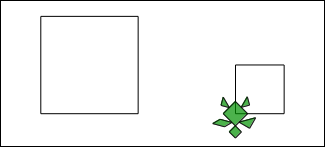
\includegraphics[width=10.0cm,trim=4 4 8 4,clip]{./images/incapsulare/incapsulare-3.png}
   \label{inc-2}
\end{figure}

\vskip 0.5cm

In realtà a noi piacerebbe controllare meglio il modo con cui vengono disegnati i quadrati, per esempio determinando la lunghezza del lato. Questo si può fare assegnando degli argomenti alla subroutine:


\vskip 0.5cm

\begin{scriptsize}
\begin{minipage}{0.50\textwidth}
\begin{itemize}[itemsep=-3pt,parsep=2pt, leftmargin=-6.0mm]
\item[] CLEARSCREEN	; operazioni di preparazione                    
\item[] HOME			; che vengono eseguite subito
\item[] SHOWTURTLE
\item[] 
\item[] ; subroutine \color{red}QUADRATO\color{black}: viene solo "imparata"...
\item[] 			        ; ma non eseguita
\item[] 
\item[] \color{green}TO \color{red}QUADRATO \color{magenta}LATO\color{black}
\item[] 	\color{blue}LATO = 100	; fisso il lato del quadrato
\item[] 	ANGOLO = 90	; angolo di rotazione ai vertici
\item[] 	FORWARD LATO	; primo lato
\item[] 	RIGHT ANGOLO	; giro di 90\degree a destra, ecc.
\item[] 	FORWARD LATO
\item[] 	RIGHT ANGOLO
\item[] 	FORWARD LATO
\item[] 	RIGHT ANGOLO
\item[] 	FORWARD LATO
\item[] \color{green}END 
\item[] 
\item[] ; script che viene eseguito
\item[] 
\item[] \color{red}QUADRATO \color{magenta}100 \color{black}		; qui si eseguono le istruzioni blu
\item[] PENUP
\item[] FORWARD 100 
\item[] PENDOWN
\item[] \color{red}QUADRATO \color{magenta}50 		; qui si eseguono le istruzioni blu         
\end{itemize}
\end{minipage}
\end{scriptsize}
\begin{minipage}{0.45\textwidth}
\color{black}Qui, dopo la dichiarazione del nome della subroutine, abbiamo introdotto l'argomento \color{magenta}LATO\color{black}. Nel codice successivo alla subroutine, l'istruzione QUADRATO viene invocata con un argomento, pari a \color{magenta}100 \color{black}la prima volta e \color{magenta}50 \color{black}la seconda. 
Ricapitolando, quando si fa eseguire il codice, premendo il tasto 
\includegraphics[height=1em]{./images/incapsulare/PlayLO.png}, LibreLogo esegue le prime tre istruzioni, poi "impara" tutte quelle contenute nella subroutine QUADRATO; quindi esegue le istruzioni sottostanti, invocando QUADRATO con un valore \color{magenta}LATO \color{black}di \color{magenta}100\color{black}, spontandosi e poi di nuovo QUADRATO con un valore di \color{magenta}LATO \color{black}di \color{magenta}50\color{black}. 
\end{minipage} \hfill

\vskip 0.5cm

Ecco il risultato:

\vskip 0.5cm

\begin{figure}[H]
   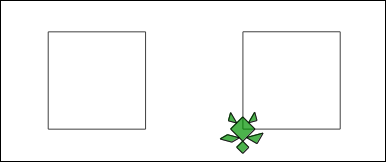
\includegraphics[width=10.0cm,trim=4 4 8 4,clip]{./images/incapsulare/incapsulare-2.png}
   \label{inc-3}
\end{figure}

\vskip 0.5cm

Così siamo liberi di invocare la nostra nuova funzione QUADRATO ogni volta che ne abbiamo bisogno, specificando liberamente la dimensione: QUADRATO 10, QUADRATO 30  o quello che vogliamo. Ora, a direil vero un'istruzione per disegnare i quadrati in LibreLogo esiste già: l'abbiamo incontrata a pag. 21, si chiama SQUARE e funziona allo stesso modo. O quasi, in realtà una differenza c'è: con SQUARE, una volta che il quadrato è stato disegnato, la tartaruga la ritroviamo al suo centro rivolta nella stessa direzione che aveva prima. Nel nostro caso invece la tartaruga rimane dove si trova dopo avere terminato di disegnare l'ultimo lato del quadrato. Effettivamente il comportamento di SQUARE sembra essere preferibile ma non è difficile far fare la stessa cosa alla nostra istruzione QUADRATO, ecco come:

\vskip 1cm

%https://en.wikibooks.org/wiki/LaTeX/Source_Code_Listings
\lstset{literate=
  {á}{{\'a}}1 {é}{{\'e}}1 {í}{{\'i}}1 {ó}{{\'o}}1 {ú}{{\'u}}1
  {Á}{{\'A}}1 {É}{{\'E}}1 {Í}{{\'I}}1 {Ó}{{\'O}}1 {Ú}{{\'U}}1
  {à}{{\`a}}1 {è}{{\`e}}1 {ì}{{\`i}}1 {ò}{{\`o}}1 {ù}{{\`u}}1
  {À}{{\`A}}1 {È}{{\'E}}1 {Ì}{{\`I}}1 {Ò}{{\`O}}1 {Ù}{{\`U}}1
  {ä}{{\"a}}1 {ë}{{\"e}}1 {ï}{{\"i}}1 {ö}{{\"o}}1 {ü}{{\"u}}1
  {Ä}{{\"A}}1 {Ë}{{\"E}}1 {Ï}{{\"I}}1 {Ö}{{\"O}}1 {Ü}{{\"U}}1
  {â}{{\^a}}1 {ê}{{\^e}}1 {î}{{\^i}}1 {ô}{{\^o}}1 {û}{{\^u}}1
  {Â}{{\^A}}1 {Ê}{{\^E}}1 {Î}{{\^I}}1 {Ô}{{\^O}}1 {Û}{{\^U}}1
  {œ}{{\oe}}1 {Œ}{{\OE}}1 {æ}{{\ae}}1 {Æ}{{\AE}}1 {ß}{{\ss}}1
  {ű}{{\H{u}}}1 {Ű}{{\H{U}}}1 {ő}{{\H{o}}}1 {Ő}{{\H{O}}}1
  {ç}{{\c c}}1 {Ç}{{\c C}}1 {ø}{{\o}}1 {å}{{\r a}}1 {Å}{{\r A}}1
  {€}{{\euro}}1 {£}{{\pounds}}1 {«}{{\guillemotleft}}1
  {»}{{\guillemotright}}1 {ñ}{{\~n}}1 {Ñ}{{\~N}}1 {¿}{{?`}}1
}
\lstset{extendedchars=true, basicstyle=\scriptsize} 
\begin{lstlisting}[frame=single]  % Start your code-block

CLEARSCREEN
HOME
SHOWTURTLE

TO QUADRATO LATO
	ANGOLO = 90		; angoli interni quadrato

	PENUP			; alzo la penna
	FORWARD LATO/2		; mi dirigo su lato che ho di fronte
				; così mi ritrovo a metà del lato 
				; di fronte
	RIGHT ANGOLO		; giro a destra
	PENDOWN			; abbasso la penna 
	FORWARD LATO/2		; disegno mezzo del primo lato 
	RIGHT ANGOLO		; giro a destra
	FORWARD LATO		; disegno il secondo lato
	RIGHT ANGOLO		; giro a destra
	FORWARD LATO		; disegno il terzo lato
	RIGHT ANGOLO		; giro a destra
	FORWARD LATO		; disegno il quarto lato
	RIGHT ANGOLO		; giro a destra
	FORWARD LATO/2		; disegno la metà rimanente del
				; quarto lato
	RIGHT ANGOLO		; giro a destra (per tornare nel
				; centro del quadrato)
	PENUP			; alzo la penna
	FORWARD LATO/2		; torno nel centro del quadrato
	LEFT ANGOLO*2		; mi rigiro nella direzione in cui 
				; mi trovavo inzialmente
END

QUADRATO 100
RIGHT 90
FORWARD 200
QUADRATO 80

\end{lstlisting}

\vskip 1cm

E questo è il risultato:

\vskip 0.5cm

\begin{figure}[H]
   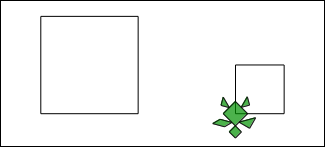
\includegraphics[width=10.0cm,trim=4 4 8 4,clip]{./images/incapsulare/incapsulare-3.png}
   \label{inc-4}
\end{figure}

\vskip 0.5cm

La tartaruga è rivolta a destra perché per disegnare il secondo quadrato ha viaggiato da sinistra verso destra. Per rendere il comportamento dell'istruzione RETTANGOLO proprio identico a quello di SQUARE si dovrebbe intervenire anche sul colore del riempimento, mentre con il codice che abbiamo scritto questo non accade. Potremmo fare anche questo, utilizzando le istruzioni FILL  e FILCOLOR, che abbiamo già visto. Lasciamo questa modifica come esercizio, per chi lo voglia fare. 
Si può obiettare che tutto questo lavoro sia inutile, visto che serve a fare una cosa che in LibreLogo già esiste. L'intento è primariamente pedagogico: le cose si spiegano bene a partire da esempi semplici; inoltre, è interessante constatare come si possano costruire da soli parti di un sistema che esistono già, perché questo ci aiuta ad acquistare fiducia e, al tempo stesso,  a rendersi conto che il sistema che stiamo usando non è chiuso e composto di una materia inaccessibile; infine, ci rendiamo conto di poter contribuire al sistema stesso, magari anche costruendo delle varianti di istruzioni preesistenti – ad esempio, potrebbe esserci utile una  versione dell'istruzione SQUARE che oltre alla dimensione del lato accetti anche il colore con il quale questo debba essere dipinto, o magari anche il colore del contorno. Qui si introduce un'altra generalizzazione: possiamo definire subroutine con più di un argomento. Per esempio possiamo provare a definire un'istruzione rettangolo, che possa essere invocata così: RETTANGOLO A B, dove A rappresenta il lato orizzontale e B quello breve. Lasciamo come esercizio le variazioni da apportare alla subroutine QUADRATO vista sopra, per ottenere una subroutine RETTANGOLO, nel modo accennato. Come lasciamo per esercizio la possibilità di introdurre il controllo dei colori, sia nella funzione QUADRATO che RETTANGOLO.
Ovviamente, se può avere senso la creazione di varianti di istruzioni esistenti, a maggio ragione, ne avrà la creazione di nuovi. Non c'è limite a quello che possiamo pensare di incapsulare in una subroutine. Prendiamo per esempio il codice che avevamo scritto a pagina 15 proviamo a incapsularlo in una subroutine:

stessa cosa alla nostra istruzione QUADRATO, ecco come:

\vskip 1cm

%https://en.wikibooks.org/wiki/LaTeX/Source_Code_Listings
\lstset{literate=
  {á}{{\'a}}1 {é}{{\'e}}1 {í}{{\'i}}1 {ó}{{\'o}}1 {ú}{{\'u}}1
  {Á}{{\'A}}1 {É}{{\'E}}1 {Í}{{\'I}}1 {Ó}{{\'O}}1 {Ú}{{\'U}}1
  {à}{{\`a}}1 {è}{{\`e}}1 {ì}{{\`i}}1 {ò}{{\`o}}1 {ù}{{\`u}}1
  {À}{{\`A}}1 {È}{{\'E}}1 {Ì}{{\`I}}1 {Ò}{{\`O}}1 {Ù}{{\`U}}1
  {ä}{{\"a}}1 {ë}{{\"e}}1 {ï}{{\"i}}1 {ö}{{\"o}}1 {ü}{{\"u}}1
  {Ä}{{\"A}}1 {Ë}{{\"E}}1 {Ï}{{\"I}}1 {Ö}{{\"O}}1 {Ü}{{\"U}}1
  {â}{{\^a}}1 {ê}{{\^e}}1 {î}{{\^i}}1 {ô}{{\^o}}1 {û}{{\^u}}1
  {Â}{{\^A}}1 {Ê}{{\^E}}1 {Î}{{\^I}}1 {Ô}{{\^O}}1 {Û}{{\^U}}1
  {œ}{{\oe}}1 {Œ}{{\OE}}1 {æ}{{\ae}}1 {Æ}{{\AE}}1 {ß}{{\ss}}1
  {ű}{{\H{u}}}1 {Ű}{{\H{U}}}1 {ő}{{\H{o}}}1 {Ő}{{\H{O}}}1
  {ç}{{\c c}}1 {Ç}{{\c C}}1 {ø}{{\o}}1 {å}{{\r a}}1 {Å}{{\r A}}1
  {€}{{\euro}}1 {£}{{\pounds}}1 {«}{{\guillemotleft}}1
  {»}{{\guillemotright}}1 {ñ}{{\~n}}1 {Ñ}{{\~N}}1 {¿}{{?`}}1
}
\lstset{extendedchars=true, basicstyle=\scriptsize}
\lstset{escapeinside={<@}{@>}}
\begin{lstlisting}[frame=single]  % Start your code-block

CLEARSCREEN	; operazioni di preparazione
HOME			; che vengono eseguite subito

; subroutine <@\textcolor{red}{CASA}@>: viene solo "imparata"...
                               ; ma non eseguita 

<@\textcolor{green}{TO}@> <@\textcolor{red}{CASA}@>
	textcolor{blue}{TO} FORWARD 50mm RIGHT 90\degree
	FORWARD 50mm RIGHT 90
	FORWARD 50mm RIGHT 90
	FORWARD 50mm RIGHT 90
	FORWARD 50mm RIGHT 30
	FILLCOLOR "yellow" FILL
	FORWARD 50mm RIGHT 120
	FORWARD 50mm RIGHT 120
	PENUP
	FORWARD 50mm/3
	LEFT 90
	FORWARD 50mm/3
	PENDOWN
	FILLCOLOR "red" FILL
	FORWARD 50mm/3 RIGHT 90
	FORWARD 50mm/3 RIGHT 90
	FORWARD 50mm/3 RIGHT 90
	FORWARD 50mm/3 RIGHT 90
	FILLCOLOR "green" FILL
	HIDETURTLE
<@\textcolor{green}{END}@>

; istruzioni eseguite

<@\textcolor{red}{CASA}@>

\end{lstlisting}

\vskip 1cm

Se si prova ad eseguire questo codice si ottiene la stessa casetta che avevamo ottenuto a pagina 15. A questo punto è facilissimo introdurre delle varianti, per esempio la dimensione delle case, che possiamo controllare mediante un'apposita variabile, che chiamiamo LATO e che passiamo come argomento nella subroutine CASA:

\vskip 1cm

%https://en.wikibooks.org/wiki/LaTeX/Source_Code_Listings
\lstset{literate=
  {á}{{\'a}}1 {é}{{\'e}}1 {í}{{\'i}}1 {ó}{{\'o}}1 {ú}{{\'u}}1
  {Á}{{\'A}}1 {É}{{\'E}}1 {Í}{{\'I}}1 {Ó}{{\'O}}1 {Ú}{{\'U}}1
  {à}{{\`a}}1 {è}{{\`e}}1 {ì}{{\`i}}1 {ò}{{\`o}}1 {ù}{{\`u}}1
  {À}{{\`A}}1 {È}{{\'E}}1 {Ì}{{\`I}}1 {Ò}{{\`O}}1 {Ù}{{\`U}}1
  {ä}{{\"a}}1 {ë}{{\"e}}1 {ï}{{\"i}}1 {ö}{{\"o}}1 {ü}{{\"u}}1
  {Ä}{{\"A}}1 {Ë}{{\"E}}1 {Ï}{{\"I}}1 {Ö}{{\"O}}1 {Ü}{{\"U}}1
  {â}{{\^a}}1 {ê}{{\^e}}1 {î}{{\^i}}1 {ô}{{\^o}}1 {û}{{\^u}}1
  {Â}{{\^A}}1 {Ê}{{\^E}}1 {Î}{{\^I}}1 {Ô}{{\^O}}1 {Û}{{\^U}}1
  {œ}{{\oe}}1 {Œ}{{\OE}}1 {æ}{{\ae}}1 {Æ}{{\AE}}1 {ß}{{\ss}}1
  {ű}{{\H{u}}}1 {Ű}{{\H{U}}}1 {ő}{{\H{o}}}1 {Ő}{{\H{O}}}1
  {ç}{{\c c}}1 {Ç}{{\c C}}1 {ø}{{\o}}1 {å}{{\r a}}1 {Å}{{\r A}}1
  {€}{{\euro}}1 {£}{{\pounds}}1 {«}{{\guillemotleft}}1
  {»}{{\guillemotright}}1 {ñ}{{\~n}}1 {Ñ}{{\~N}}1 {¿}{{?`}}1
}
\lstset{extendedchars=true, basicstyle=\scriptsize} 
\begin{lstlisting}[frame=single]  % Start your code-block

CLEARSCREEN
HOME

<@\textcolor{green}{TO}@> <@\textcolor{red}{CASA}@> <@\textcolor{magenta}{LATO}@>
	FORWARD LATO RIGHT 90\degree
	FORWARD LATO RIGHT 90
	FORWARD LATO RIGHT 90
	FORWARD LATO RIGHT 90
	FORWARD LATO RIGHT 30
	FILLCOLOR "yellow" FILL
	FORWARD LATO RIGHT 120
	FORWARD LATO RIGHT 120
	PENUP
	FORWARD LATO/3
	LEFT 90
	FORWARD LATO/3
	PENDOWN
	FILLCOLOR "red" FILL
	FORWARD LATO/3 RIGHT 90
	FORWARD LATO/3 RIGHT 90
	FORWARD LATO/3 RIGHT 90
	FORWARD LATO/3 RIGHT 90
	FILLCOLOR "green" FILL
	HIDETURTLE
<@\textcolor{green}{END}@>


PENUP POSITION [150,400] HEADING 0 PENDOWN
<@\textcolor{red}{CASA}@> <@\textcolor{magenta}{30mm}@>
PENUP POSITION [200,400] HEADING 0 PENDOWN
<@\textcolor{red}{CASA}@> <@\textcolor{magenta}{30mm}@>
PENUP POSITION [270,400] HEADING 0 PENDOWN
<@\textcolor{red}{CASA}@> <@\textcolor{magenta}{30mm}@>

\end{lstlisting}

\vskip 1cm

Il codice della subroutine \color{red}CASA \color{black}è lo stesso di prima eccetto per la presenza dell'argomento \color{magenta}LATO\color{black}. Nello script l'istruzione \color{red}CASA \color{black}viene chiamata tre volte, sempre con dimensioni diverse. La posizione viene controllata mediante sequenze di istruzioni del tipo \textbf{PENUP POSITION [150,400] HEADING 0 PENDOWN}: alzo la penna, mi trasferisco nel punto di coordinate [150,400] (peer esempio), mi dirigo in su, riabbasso la penna. Ecco il risultato:

\vskip 0.5cm

\begin{figure}[H]
   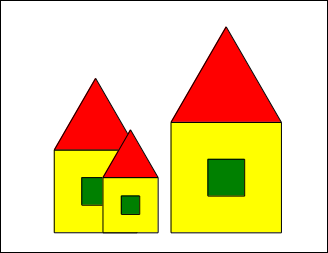
\includegraphics[width=10.0cm,trim=4 4 8 4,clip]{./images/incapsulare/incapsulare-4.png}
   \label{inc-5}
\end{figure}

\vskip 0.5cm

Non c'è limite alla fantasia. Non è difficile scrivere una subroutine che disegni un albero e usarla per arricchire così il paesaggio. Lo proponiamo come esercizio dopo, ma prima vediamo un altro esempio più avanzato, intendendo con questo che potrebbe essere utilizzato in un contesto di scuola secondaria superiore (la descrizione che segue è molto dettagliata, chi non è interessato a un contesto del genere e non ha dimestichezza con questo livello di conoscenza matematiche, salti senz'altro l'esempio!). Riprendiamo le successioni di poligoni che avevamo visto a pag. 45 e 46. Lì avevamo rappresentato la successione incolonnando i poligoni. L'idea ora è di sovrapporli anziché incolonnarli, in modo da apprezzare l'evoluzione verso il cerchio al crescere del numero dei lati. Scegliamo di costruire i poligoni inscritti in un cerchio di raggio dato, formando così la successione dei poligoni inscritti nel cerchio. Potremmo egualmente considerare la successione dei poligoni circoscritti al cerchio. Nel primo caso il parametro chiave è il raggio dei poligoni, sempre eguale al raggio del cerchio in cui sono inscritti. Nel secondo sarebbe invece l'apotema, sempre eguale al raggio del cerchio che circoscrivono. L'esempio che segue descrive il primo caso. Il codice che segue è commentato minuziosamente. Ciò nonostante descriviamo puntualmente la struttura del codice e il procedimento. 
 Intanto l'esercizio utilizza, in un contesto un po' più complicato, i tre
 costrutti fondamentali del software che abbiamo sin qui introdotto: le
 variabili e le operazioni fra di esse, le ripetizioni di sequenze di
 istruzioni e l'incapsulamento di sezioni di codice nelle subroutine. Abbiamo
 mantenuto l'evidenziazione cromatica che abbiamo usato in alcuni degli esempi
 precedenti, per aiutare la lettura del codice. Nella prima sezione(in nero) si
 eseguono le operazioni preparatorie: cancellazione del foglio, tartaruga a
 casa, tartaruga invisibile (sarebbe troppo "invasiva" su un disegno più
 articolato come questo), penna alzata; inoltre si fissano i parametri
 necessari per iniziare, ovvero numero dei poligoni che dovranno comporre la
 successione, e raggio dei poligoni, espresso in punti. Poi viene il codice
 della subroutine textbf{POLIGONO}, con le istruzioni in blu, eccetto il nome
 della subroutine in rosso e i suoi argomenti in viola. La subroutine
 textbf{POLIGONO} richiede 5 argomenti: X0P e Y0P sono le coordinate del centro
 del poligono, che possiamo quindi piazzare dove vogliamo; N è il numero di
 lati che deve avere il poligono; R è il raggio del poligono. All'interno della
 subroutine textbf{POLIGONO} si sviluppa la geometria. Si calcola l'ampiezza
 degli angoli interni \textbf{AI}, l'ampiezza degli angoli supplementari degli
 angoli \textbf{AI}, che chiamiamo A e la lunghezza dei lati \textbf{L}. Qui
 troviamo una novità, anzi due: \textbf{SIN} e \textbf{ABS} sono funzioni
 matematiche e \textbf{PI} è una costante. Scopriamo quindi che LibreLogo "sa"
 un bel po' di matematica! \textbf{PI} è una variabile speciale, per meglio
 dire una costante, la più importante della matematica: il $\pi$ (pi greco), di cui
 LibreLogo esprime un'approssimazione con 15 cifre decimali (provare ad
 eseguire l'istruzione \textbf{PRINT PI})\footnote{Ricordiamo che  $\pi$
 rappresenta il rapporto fra la misura della circonferenza e il raggio di un
 cerchio, e che si tratta di numero irrazionale, quindi con un numero infinito
 di cifre decimali.}. Invece \textbf{SIN} e \textbf{ABS}
 sono funzioni matematiche: \textbf{SIN} calcola il valore della funzione
 trigonometrica seno e richiede un argomento espresso in radianti, per esempio
 \textbf{SIN PI} fornisce il valore \textbf{0}; \textbf{ABS} calcola il valore
 assoluto dell'argomento, ovvero se è positivo lo lo lascia positivo mentre se
 è negativo lo trasforma in positivo. Successivamente vengono le istruzioni che
 disegnano il poligono, ovvero il viaggio della tartaruga. In sintesi, la
 tartaruga va nel centro indicato, di coordinate \textbf{[X0P, Y0P]}, si volge
 in alto e percorre senza disegnare il raggio, gira a destra di 90\degree (questa è
 la direzione della tangente al cerchio circoscritto), poi gira di quanto basta
 per allinearsi al primo lato del  poligono (si poteva girare in un sol colpo
 verso questa direzione, ma abbiamo lasciato il codice in questa forma
 sotto-ottimale per chiarire la geometria). A questo punto si abbassa la penna
 e si iniziano a disegnare i lati in successione, mediante il semplice ciclo
 \textbf{REPEAT N [FORWARD L RIGHT A]}. Le istruzioni finali all'interno della
 subroutine servono a scrivere un'etichetta, poco sotto al centro del poligono,
 con il numero di lati. Siccome è un codice che ci mette un certo tempo girare
 (ovviamente questo dipende anche dal computer che si usa), quando il numero di
 lati diventa elevato, è utile per sapere a che punto si trova il processo –
 noi abbiamo provato fino a 500 lati. Da segnalare qui l'uso della variabile
 riservata (in LibreLogo) di \textbf{REPCOUNT}, che è il contatore di cicli.
 Inoltre, si usa la funzione \textbf{STR} che serve a trasformare il valore di
 \textbf{REPCOUNT}, che è un numero espresso internamente al computer in
 binario, nell'espressione alfanumerica del medesimo, che possa essere stampata
 sul foglio come qualsiasi altro testo\footnote{Questa è una nozione che a
 qualcuno può sembrare oscura. Molto in sintesi: una cosa sono i numeri
 espressi in un formato con il quale il computer possa fare i calcoli e
 un'altra sono i numeri espressi come caratteri, che possono essere
 inframezzati in un testo qualsiasi. Nel primo caso si tratta di una codifica
 per il computer è binaria, l'unico modo che consenta al computer di fare
 operazioni matematiche. Nel secondo di tratta di una codifica che serve a
 rappresentare i caratteri sullo schermo, o in una stampa; questa è una
 codifica che ha una finalità puramente grafica e che il computer non può usare
 per fare i calcoli. Esistono molti tipi di codifiche, le più note della quali
 sono ASCII E UNICODE. Chi desidera chiarimenti si può rivolgere all'autore di
 questo testo.}. La stampa dell'etichetta è subordinata
 la fatto che si tratti dell'ultimo poligono. Questo controllo viene effettuato
 con l'istruzione di controllo \textbf{IF}, descritta nel capitolo successivo.
 Dopo il codice della subroutine, di nuovo in nero, c'è lo script vero e
 proprio, molto semplice. Le tre istruzioni \textbf{HOME, X0P=POSITION[0]} e
 \textbf{Y0P=POSITION[1]} servono per piazzare il centro dei poligoni nel
 centro del foglio, ma qui potremmo scegliere una qualsiasi altra posizione.
 Infine, la realizzazione della successione è affidata al ciclo
 \textbf{REPEAT NP […]}. Anche qui si usa il contatore di cicli, in questo
 caso, per chiamare la subroutine POLIGONO con il giusto numero di lati. Come
 dicevamo, questo script può richiedere del tempo, se fatto girare con un
 numero elevato di poligoni, diciamo da 10 in su, indipendenza della velocità
 del processore che equipaggia il computer. Se capita di farlo partire
 inavvertitamente con un numero di lati eccessivo, o se lo si vuole fermare per
 qualsiasi altro motivo, lo si può fare con il
 tasto
\includegraphics[height=1em]{./images/ripetere/StopLO.png}. Se si supera il valore di circa 30 lati, si inizia a vedere un contorno apparentemente circolare. Più che si aumenta il numero di lati e più che la circolarità è "vera".


\vskip 1cm

%https://en.wikibooks.org/wiki/LaTeX/Source_Code_Listings
\lstset{literate=
  {á}{{\'a}}1 {é}{{\'e}}1 {í}{{\'i}}1 {ó}{{\'o}}1 {ú}{{\'u}}1
  {Á}{{\'A}}1 {É}{{\'E}}1 {Í}{{\'I}}1 {Ó}{{\'O}}1 {Ú}{{\'U}}1
  {à}{{\`a}}1 {è}{{\`e}}1 {ì}{{\`i}}1 {ò}{{\`o}}1 {ù}{{\`u}}1
  {À}{{\`A}}1 {È}{{\'E}}1 {Ì}{{\`I}}1 {Ò}{{\`O}}1 {Ù}{{\`U}}1
  {ä}{{\"a}}1 {ë}{{\"e}}1 {ï}{{\"i}}1 {ö}{{\"o}}1 {ü}{{\"u}}1
  {Ä}{{\"A}}1 {Ë}{{\"E}}1 {Ï}{{\"I}}1 {Ö}{{\"O}}1 {Ü}{{\"U}}1
  {â}{{\^a}}1 {ê}{{\^e}}1 {î}{{\^i}}1 {ô}{{\^o}}1 {û}{{\^u}}1
  {Â}{{\^A}}1 {Ê}{{\^E}}1 {Î}{{\^I}}1 {Ô}{{\^O}}1 {Û}{{\^U}}1
  {œ}{{\oe}}1 {Œ}{{\OE}}1 {æ}{{\ae}}1 {Æ}{{\AE}}1 {ß}{{\ss}}1
  {ű}{{\H{u}}}1 {Ű}{{\H{U}}}1 {ő}{{\H{o}}}1 {Ő}{{\H{O}}}1
  {ç}{{\c c}}1 {Ç}{{\c C}}1 {ø}{{\o}}1 {å}{{\r a}}1 {Å}{{\r A}}1
  {€}{{\euro}}1 {£}{{\pounds}}1 {«}{{\guillemotleft}}1
  {»}{{\guillemotright}}1 {ñ}{{\~n}}1 {Ñ}{{\~N}}1 {¿}{{?`}}1
}
\lstset{extendedchars=true, basicstyle=\scriptsize}
\lstset{escapeinside={<@}{@>}}
\begin{lstlisting}[frame=single]  % Start your code-block

; Script per disegnare una successione di poligoni inscritti in un 
; cerchio di raggio R dato

CLEARSCREEN		; pulisco il foglio
HOME			; tartaruga a casa
HIDETURTLE		; tartaruga invisibile
PENUP			; alzo la penna
NP = 20			; numero poligoni
R = 100			; raggio poligoni - tengo fisso il raggio per  
			; tutti i poligoni
			; cosicché risultano tutti inscritti nello 
			; stesso cerchio di raggio R
; subroutine POLIGONO
; 	argomenti:	X0P: X del centro del poligono	
;			Y0P: Y del centro del poligono
;			N: numero lati poligono
;			R: misura raggio
;			NP: numero poligoni (serve a scrivere 
;			    l'etichetta)

<@\textcolor{green}{TO}@> <@\textcolor{red}{POLIGONO}@> <@\textcolor{magenta}{X0P}@> <@\textcolor{magenta}{Y0P}@> <@\textcolor{magenta}{N}@> <@\textcolor{magenta}{R}@> <@\textcolor{magenta}{NP}@>
 	A = 360/N			; angoli supplementari degli 
					; angoli interni: quelli 
					; di cui gira
					; la tartaruga ad ogni vertice  
					; (N -> infinito => A -> 0)
	AI = 180*(N-2)/N		; angoli interni  
					; (N -> infinito => AI -> 180)
	L = ABS(2*R*SIN(A/2*PI/180))	; lato

;	Disegno il poligono

	FILLCOLOR "white" PENDOWN CIRCLE 3 PENUP
	POSITION [X0P,Y0P]		; vado al centro
	HEADING 0			; mi dirigo in su
	FORWARD R			; percorro il raggio
	RIGHT 90			; 90 gradi a destra (direzione 
					; tangente al cerchio 
					; circoscritto)
	RIGHT (180 - AI)/2		; direzione primo lato da 
					; disegnare
	PENDOWN				; giù la penna
	REPEAT N [			; ciclo sui lati del poligono
		FORWARD L RIGHT A
	]
	PENUP				; alzo la penna
	POSITION [X0P,Y0P]		; torno al centro 
	IF REPCOUNT = NP [
		FORWARD 10		; vado un po' sotto per 
					; scrivere etichetta
		HEADING 0			; mi giro in su per...
		LABEL "N = " + STR REPCOUNT	; ... scrivere etichetta 
						; corrente 
		HEADING 6h			; mi rigiro in giù
		BACK 10				; torno al centro
	]
<@\textcolor{green}{END}@>			; fine subroutine POLIGONO

; script vero e proprio

HOME					; vado al centro ma potrei 
					; andare anche altrove 
X0P = POSITION[0]			; X del centro del poligono
Y0P = POSITION[1]			; Y del centro del poligono
REPEAT NP [				; ciclo sui poligoni
	N = REPCOUNT+2			; numero lati poligono
	POLIGONO X0P Y0P N R NP
]


\end{lstlisting}

\vskip 1cm

Ecco il risultato:

\vskip 0.5cm

\begin{figure}[H]
   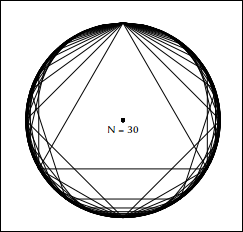
\includegraphics[width=7.0cm,trim=4 4 8 4,clip]{./images/incapsulare/incapsulare-5.png}
   \label{inc-6}
\end{figure}

\vskip 0.5cm

Dove sono sovrapposti i poligoni regolari, a partire dal triangolo equilatero (N=3), fino a quello con 30 lati. 

\subsubsection{Esercizio}

Riprendendo l'esempio della costruzione di case con un'apposita subroutine, si provi ad arriccchire il paesaggio...

\vskip 0.5cm

\begin{figure}[H]
   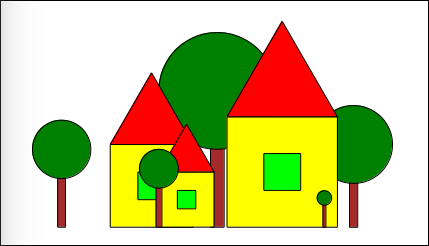
\includegraphics[width=10.0cm,trim=4 4 8 4,clip]{./images/incapsulare/incapsulare-6.png}
   \label{inc-7}
\end{figure}

\vskip 0.5cm


